\documentclass[a4paper]{slides}

\usepackage{tikz}
\usepackage{geometry}

\usepackage[scaled]{helvet}
\usepackage[T1]{fontenc}

% Set Layout
\geometry{
    a4paper,
    left=25mm,
    right=25mm,
    top=25mm,
    bottom=25mm
}

\begin{document}

\fontsize{15}{1.5}\textbf{Bitte in Schreibrichtung die Großbuchstaben von A bis Z eintragen}

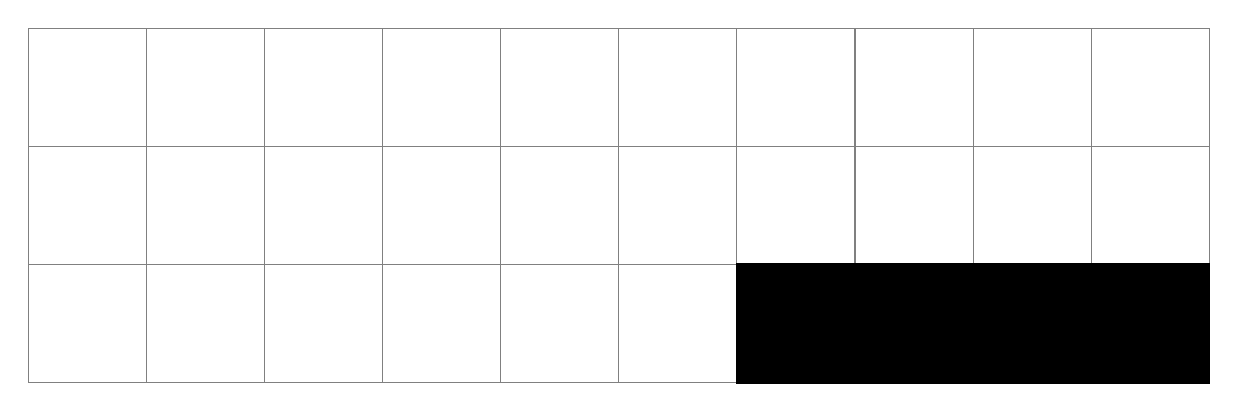
\begin{tikzpicture}[thick, scale=1.5]
    \draw[step=1cm,gray,thin] (0,0) grid (10,3);
    \filldraw[fill=black, draw=black] (6,0) rectangle (7,1);
    \filldraw[fill=black, draw=black] (7,0) rectangle (8,1);
    \filldraw[fill=black, draw=black] (8,0) rectangle (9,1);
    \filldraw[fill=black, draw=black] (9,0) rectangle (10,1);
\end{tikzpicture}

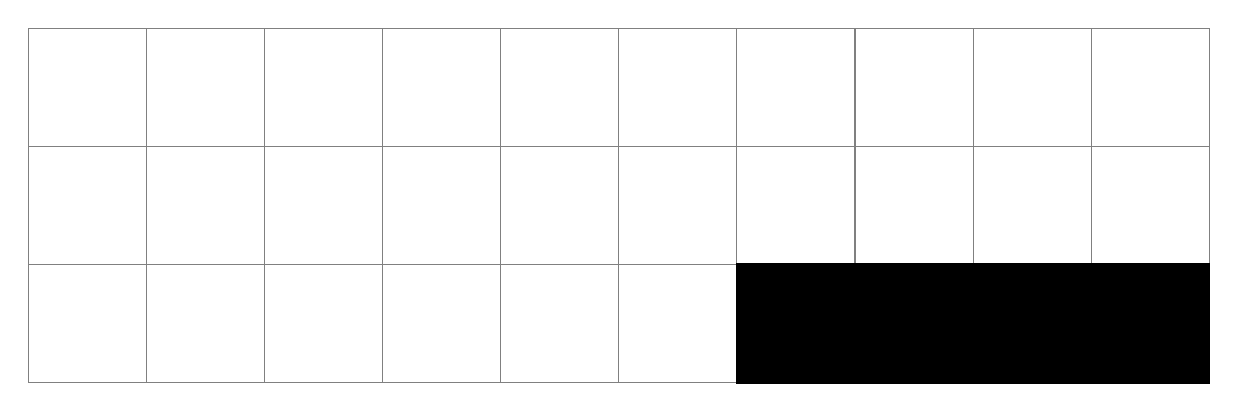
\begin{tikzpicture}[thick, scale=1.5]
    \draw[step=1cm,gray,thin] (0,0) grid (10,3);
    \filldraw[fill=black, draw=black] (6,0) rectangle (7,1);
    \filldraw[fill=black, draw=black] (7,0) rectangle (8,1);
    \filldraw[fill=black, draw=black] (8,0) rectangle (9,1);
    \filldraw[fill=black, draw=black] (9,0) rectangle (10,1);
\end{tikzpicture}

\fontsize{15}{1.5}\textbf{Bitte in jede reihe die Zahlen von 0 bis 9 eintragen }

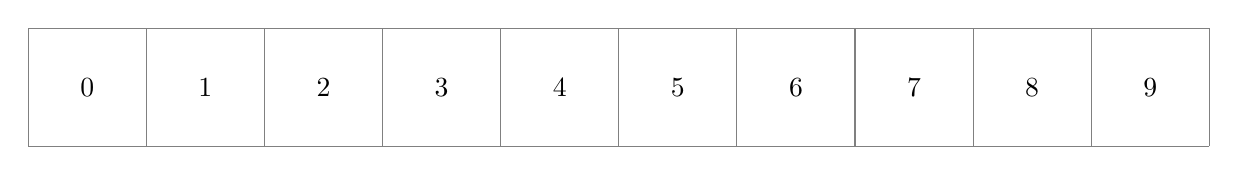
\begin{tikzpicture}[thick, scale=1.5]
    \draw[step=1cm,gray,thin] (0,0) grid (10,1);
    \node[anchor = center] () at (0.5,0.5){0};
    \node[anchor = center] () at (1.5,0.5){1};
    \node[anchor = center] () at (2.5,0.5){2};
    \node[anchor = center] () at (3.5,0.5){3};
    \node[anchor = center] () at (4.5,0.5){4};
    \node[anchor = center] () at (5.5,0.5){5};
    \node[anchor = center] () at (6.5,0.5){6};
    \node[anchor = center] () at (7.5,0.5){7};
    \node[anchor = center] () at (8.5,0.5){8};
    \node[anchor = center] () at (9.5,0.5){9};
\end{tikzpicture}

\begin{tikzpicture}[thick, scale=1.5]
    \draw[step=1cm,gray,thin] (0,0) grid (10,5);
\end{tikzpicture}

\end{document}
